%%%%%%%%%%%%%%%%%%%%%%%%%%%%%%%%%%%%
% This is the template for submission to HPCA 2016
% The cls file is a modified from  'sig-alternate.cls'
%%%%%%%%%%%%%%%%%%%%%%%%%%%%%%%%%%%%

\documentclass{sig-alternate}
\usepackage{mathptmx} % This is Times font

\newcommand{\ignore}[1]{}
\usepackage{fancyhdr}
\usepackage[normalem]{ulem}
\usepackage[hyphens]{url}
\usepackage{hyperref}
\usepackage{multirow}


%%%%%%%%%%%---SETME-----%%%%%%%%%%%%%
\newcommand{\hpcasubmissionnumber}{NaN}
 \newcommand{\tabincell}[2]{\begin{tabular}{@{}#1@{}}#2\end{tabular}}
%%%%%%%%%%%%%%%%%%%%%%%%%%%%%%%%%%%%


%%%%%%%%%%%---SETME-----%%%%%%%%%%%%
\title{vNUIOA: Optimizing Non-Uniform I/O Access in Virtualized Environment for Multicore Systems}
\author{Jianmin Qian Jian Li Junshen Tan Yangde Li Zhiyuan Bo}
%%%%%%%%%%%%%%%%%%%%%%%%%%%%%%%%%%%%

\begin{document}
\maketitle

\pagestyle{plain}

\begin{abstract}

This document is intended to serve as a sample for submissions to HPCA 2016. We provide some guidelines that authors should follow when submitting papers to the conference. In an effort to respect the efforts of reviewers and in the interest of fairness to all prospective authors, we request that all submissions follow the formatting and submission rules detailed below.

\end{abstract}

\section{Introduction}
Driven by the rapid growth of big data applications and cloud computing, most of today's applications are computing intensive or data intensive and these applications are running in the cloud to make full use of multi-core resources. To efficiently transfer data between high performance servers and these cloud applications become significantly important. Especially in the current high performance network environment, such inefficiency will cause huge performance degradation. However, the underlying topology of multi-core systems and virtualization pose great challenge in solving this problem. Several observations of performance degradation are reported because of hardware resources affinity[1, 2, 3]. Existing researches focusing on the memory locality [4, 5, 6] to reducing the remote access and virtual machine scheduling to minimize uncore penalty [7, 8, 9].

Each CPU socket accesses faster to the directly attached hardware devices than the remote ones, such as Non-Uniform memory Access (NUMA). However, directly attached devices are not limited to memory and CPU, I/O devices such as high speed Ethernet network adapter also connect to the CPU socket through the interconnect bus. When a thread access I/O devices remotely, latency will increased and inter-node maximum bandwidth decreased. This access asymmetry becomes main bottleneck of today��s high performance computing. Especially in the current high performance virtualized environment such as Network Function Virtualization (NFV)[], I/O latency in the host NUMA machine can cause a huge performance degradation of the latency sensitive NFV workloads, which are running in the virtual machines (VMs). This significantly impacts the performance data center infrastructures.
%We run Netperf benchmark on two of the same Intel 4-sockets NUMA machine, one is server other is client, with the KVM virtual machine monitor running on the server. We use the client to drive a TCP\_STREAM profile with different message sizes.

%Figure 1 shows a Four-sockets Intel Ivy Bridge NUMA architecture with a 40 Gigabit Ethernet adapter. We simply run number of virtual machines based on this architecture by varying vCPUs and memory mappings among the multiple sockets. First, we banding all the VM vCPUs to the specific core on the socket 0 and mapping all the memory of the VM to the memory bank attached to socket 0 (mark as red process), then we changed the vCPUs banding to the socket 2 and memory mapping to the socket 2 (mark as green process). Traditionally, these are both NUMA local assess, we observe a huge I/O performance difference between this two kinds of NUMA local access, I/O Throughtput of the first kind mapping is average 35.1\% (max up to 68.1\%)higher than the second kind. The main reason of this performance degradation is that when transfer data with network adapter, the second kind mapping is I/O device remote access and need to use two hops interconnection between sockets, this increase the bandwidth consumption and access latency. Recent works also has realize this problem, study [10] introduce the overheads of high Speed database query processing over this architecture in the high speed networks. work [11] also characterize the I/O bandwidth performance models of data intensive applications.
%\begin{figure}[tb]
%\centering
%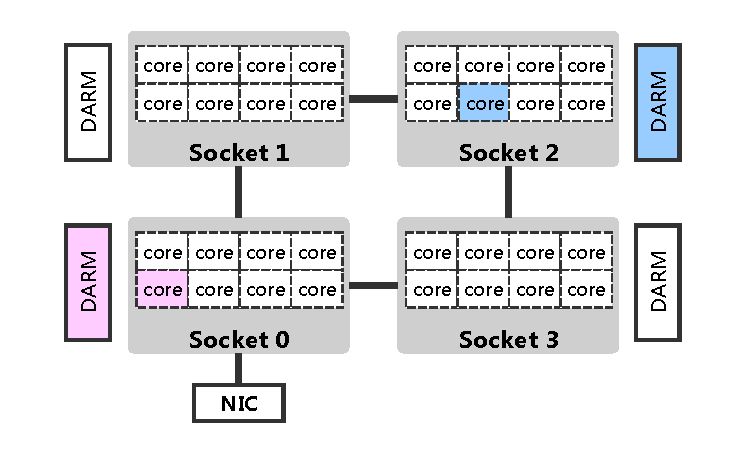
\includegraphics[width=3.5in]{Test1.pdf}
%\vspace{-2.0em}
%\caption{Two kinds of NUMA remote access.}
%\vspace{-1.0em}
%\label{fig_sim}
%\end{figure}

Although previous studies presented several affinity models to optimizing NUMA system, these models are not suitable for current high performance virtualized environment for following reasons.

%This document is intended to serve as a sample for submissions to HPCA 2016. It is heavily derived from previous conferences, in particular MICRO 2015.

%We provide some guidelines that authors should follow when submitting papers to the conference. \textbf{This format is derived from the ACM \texttt{sig-alternate.cls} file, with the major difference that it is 10pt Times font}.

%In an effort to respect the efforts of reviewers and in the interest of fairness to all prospective authors, we request that all submissions follow the formatting and submission rules detailed below. Submissions that (grossly) violate these instructions may not be reviewed, at the discretion of the Program Chair, in order to maintain a review process that is fair to all potential authors.
%In a nutshell:
\vspace{1ex}

\begin{itemize}
\item Existing NUMA affinity models are 2-dimension and mainly focusing on the memory and virtual CPU locality, the consideration of high speed interconnections affinity such as I/O devices locality are poor. since almost the cloud space applications frequent transfer data with high speed I/O devices, current affinity model must take I/O devices into consideration.
\item Many traditional NUMA performance model use the hop distance to introduce the access penalty between two devices. However, hop distance is not accurate for modeling, especially for the I/O performance modeling due to: First, the hop distance contain less details about the underlying topology such as the access latency, so it can not be used in the accurate performance measurement. Second, hop distance always be a constant in the system. When the performance of the system changing in real time, the hop distance can not reflect this change and cause the performance prediction inaccurate.
\item Furthermore, previous work only optimizing the Non-Uniform I/O access by performance tuning. They just binding the virtual machine threads and its memory together to the I/O device attached nodes to ensure local I/O access. This static method is not always efficient because too many threads in one node will increase the CPU load and hurt the performance significantly when the system load is too high.
%\item References must include all authors to facilitate the reviewing process (no \emph{et al.})Papers must be at most 11 pages, not including references, in two-column format.Paper must be submitted in printable PDF format.Text must be minimum 10pt Times font.
%\item There is no page limit for references.

\end{itemize}
In this paper, we present a novel locality model, vNUIOA, which mainly optimizing IO locality in the high performance virtualized system and both taking thread to thread affinity in to consideration. We first install SR-IOV technology into our system to providing high performance I/O virtualization, then we implement a hardware monitor by change the performance monitor units (PMU) both in physical machine and virtual machines. Based on the PMU hardware resource usages such as IO requests, VM address distribution and CPU utilization, we analyzed
We evaluated our model on Intel multi-core machine and conduct a series of experimental. Results show that

The contributions of this paper include:

This paper is organized as follows: Section 2 provides an overview of NUIOA architecture, I/O virtualization technology and motivation for this research. Section 3 characterizes performance in NUIOA virtualized systems. Sections 4 and 5 present our design and implementation. Section 6 evaluates our prototype and compares with existing methods.Section 7 discusses related work and Section 8 concludes this paper.

\section{Background and Motivation}
In this section, we begin with a brief introduction to asymmetric access architecture in multicore systems, Then we show performance degradation due to asymmetric access in high performance network environment. Lastly, we talk about that virtualization also aggravate the performance degradation.
\subsection{Asymmetric Access in Multicore Syetems}
%Performance Degradation in NUMA Architecture with High Speed Network Adapter
\textbf{\emph{Asymmetric Memory Access}}:Traditional multicore processor shared with one memory controller. With the number of cores per socket increases, one memory controller results in high memory controller contention and bandwidth competition. In order to improve the utilization of multicore system, each CPU socket has been designed with its own integrated memory controller (IMC) which have faster access to local memory bank than the remote ones. This Non-Uniform Memory Access (NUMA) characteristic fully take advantage of multicore system and high speed memory bandwidth.

%In order to move data fast enough to keep up with today's processors in the virtualized system, I/O devices also should be virtualized and to be shared by multiple virtual machines. In traditional para-virtualization, when a guest VM accesses the I/O device, VMM needs to intervene the data processing to share the physical device. this extra VMM intervention bring additional overhead which tremendously affect the I/O performance of guest VMs. Single Root I/O virtualization (SR-IOV) [] proposes a set a hardware enhancements for PCIe device. SR-IOV enable to create multiple "lightweight" PCIe functions,known as virtual Functions (VFs) that still contain the major device resources. In this work, we mainly consider SR-IOV because With the hardware enhancement, SRIOV remove the major VMM intervention and achieve I/O virtualization without losing performance.

%With the data transfer speed of current network adapter become higher and higher, such as Mellanox 40,56 and 100 Gigabit Ethernet adapter [] is being adopted broadly in the data center. The speed of these network adapter is higher than the memory bandwidth and resulting in shifting system bottleneck from remote memory access to asymmetric I/O access in the NUMA architecture.
\textbf{\emph{Asymmetric I/O Access}}:Besides the asymmetric memory access, this architecture also result in asymmetric accesses of other devices. One of the most important one is I/O devices, because I/O devices are also directly connected to one or more nodes in the multicore system. local cores and devices have privilegiert access to the I/O device, remote ones must use interconnection to transfer data to the I/O devices, resulting in extra inter-node bandwidth occupation and access latency. This asymmetry I/O access is called Non-Uniform I/O Access (NUIOA)[]. AMD processors have exhibited NUIOA effects when AMD introduced the OPTERON processor in 2003 [], Intel processors have began to appear NUIOA characteristic when the advent of \emph{sandy-bridge} architecture in 2011 []. Figure 1 shows a ubiquitous four-sockets NUIOA architecture based on the Intel Xeon E5 Family processors. Each socket consists of eight cores that share the last level cache (L3 cache), memory controller and physical memory bank. sockets link with each other via a high-speed, point-to-point interconnection such as Intel Quick Path Interconnect (QPI)[]. Network adapter is directly attached to the socket 0 with the Intel Data Direct I/O (DDIO) technology [], consequently, data transfer remotely to other sockets and increase access latency and bandwidth consumption.

\begin{figure}[h]
\centering
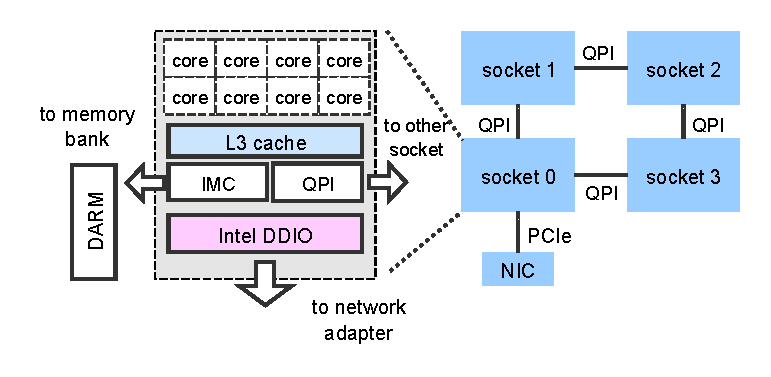
\includegraphics[width=3.5in]{NUIOA-arch.pdf}
\vspace{-1em}
\caption{Asymmetric I/O access architecture with four 8-cores Intel Xeon E5-4610 processors.}
\vspace{-1em}
\label{fig_sim}
\end{figure}
%In order to move data fast enough to keep up with today's processors in the virtualized system, I/O devices also should be virtualized and to be shared by multiple virtual machines. In traditional para-virtualization, when a guest VM accesses the I/O device, VMM needs to intervene the data processing to share the physical device. this extra VMM intervention bring additional overhead which tremendously affect the I/O performance of guest VMs. Single Root I/O virtualization (SR-IOV) [] proposes a set a hardware enhancements for PCIe device. SR-IOV enable to create multiple "lightweight" PCIe functions,known as virtual Functions (VFs) that still contain the major device resources. In this work, we mainly consider SR-IOV because With the hardware enhancement, SRIOV remove the major VMM intervention and achieve I/O virtualization without losing performance.
%\begin{figure}[tb]
%\centering
%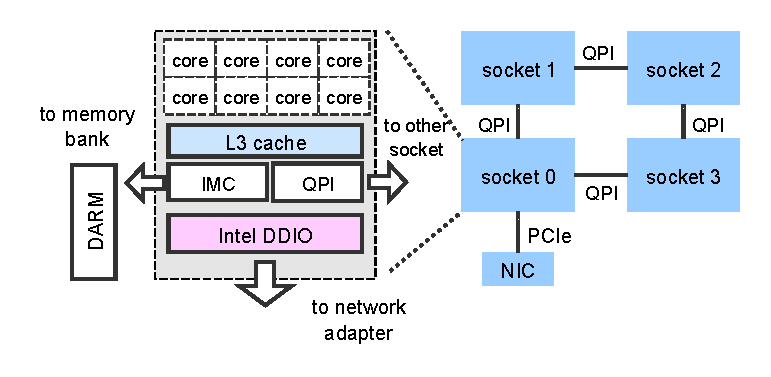
\includegraphics[width=3.5in]{NUIOA-arch.pdf}
%\vspace{-1em}
%\caption{NUIOA architecture with four 8-cores Intel Xeon E5-4610 processors.}
%\vspace{-1em}
%\label{fig_sim}
%\end{figure}

\subsection{Performance Degradation Due to Asymmetric Access}
%With the data transfer speed of current network adapter become higher and higher, such as Mellanox 40,56 and 100 Gigabit Ethernet adapter [] is being adopted broadly in the data center. The speed of these network adapter is higher than the memory bandwidth and resulting in shifting system bottleneck from remote memory access to asymmetric I/O access in the NUMA architecture. I/O device is directly connected to one or more nodes in the multicore system, local cores and devices have privilegiert access to the I/O device, remote ones must use interconnection to transfer data to the I/O devices, resulting in extra inter-node bandwidth occupation and access latency. This asymmetry I/O access is called Non-Uniform I/O Access (NUIOA). Figure 2 shows a ubiquitous four-sockets NUIOA architecture based on the Intel Xeon E5 Family processors. Each socket consists of eight cores that share the last level cache (L3 cache), memory controller and physical memory bank. sockets link with each other via a high-speed, point-to-point interconnection such as Intel Quick Path Interconnect (QPI)[]. Network adapter is directly attached to the socket 0 with the Intel Data Direct I/O (DDIO) technology [] which could directly sent data to the cache instead of memory, consequently, data transfer remotely to other sockets and increase access latency and bandwidth consumption.
\subsubsection{Moving from 10GbE to 40GbE}
With the data transfer speed of current network adapter become higher and higher, such as Mellanox 40 and 56 Gigabit Ethernet adapter [] is being adopted broadly in the data center. The speed of these network adapter is higher than the memory and interconnection bandwidth, and result in shifting of system bottleneck from asymmetric memory access to asymmetric I/O access in the NUMA architecture. Finally, without consideration of the asymmetric I/O access in high speed networking environment, the performance of data center servers degrade significantly. To measure the Performance degradation due to asymmetric access, we conduct a set of experiments. First we evaluate the performance degradation of asymmetric I/O Access independently, then we combine asymmetric memory access and asymmetric I/O access and study the factors of performance degradation.

Table 1 shows the configuration details of our test hardware. We select Netperf [] benchmark provides network bandwidth testing between two host on a network.

\begin{table}[h]
\caption{Configuration details of our test server.}

\begin{tabular}{|l|l|}
\hline
Item &
Configuration \\
\hline
CPU &
\tabincell{l}{Intel Xeon E5-4610 v2\\2.3GHz (8 cores)} \\
\hline
Memory  &
\tabincell{l}{128G RAM DDR3\\ 4 sockets, each with 32GB}\\
\hline
QPI  &
7.2 GT/s, 2 links \\
\hline
Network Adapter &
\tabincell{l}{Mellanox ConnectX-3 Dual-Port\\40 Gigabit Ethernet adapter}\\
\hline
Hypervisor &
KVM 2.0.0\\
\hline
\end{tabular}

\end{table}
\subsubsection{Evaluation of Asymmetric I/O Access}
To study the impact on performance of asymmetric I/O access independently, the VM vCPU and memory should be mapping to the same node to ensure local memory access. we simply run a number of VMs based on the asymmetric I/O access architecture by varying vCPU and memory mappings together among the multiple sockets. As shown in figure 2, a Four-sockets Intel Ivy Bridge NUMA architecture with ethernet adapter. Firstly, we banding vCPU of the VM to a specific core on the socket 0 and mapping all the memory of the VM to the memory bank attached to socket 0, then we change the VM vCPU banding to the core on the socket 2 and mapping memory of VM to the socket 2. Traditionally, these two kinds of mapping strategy ensure the VM vCPU thread is locally access to the VM memory, so the affinity between VM vCPU and memory can achieve best. However, we observe a huge I/O performance difference between this two kinds of VM vCPU and memory mapping strategy by using the Netperf benchmark.

\begin{figure}[tb]
\centering
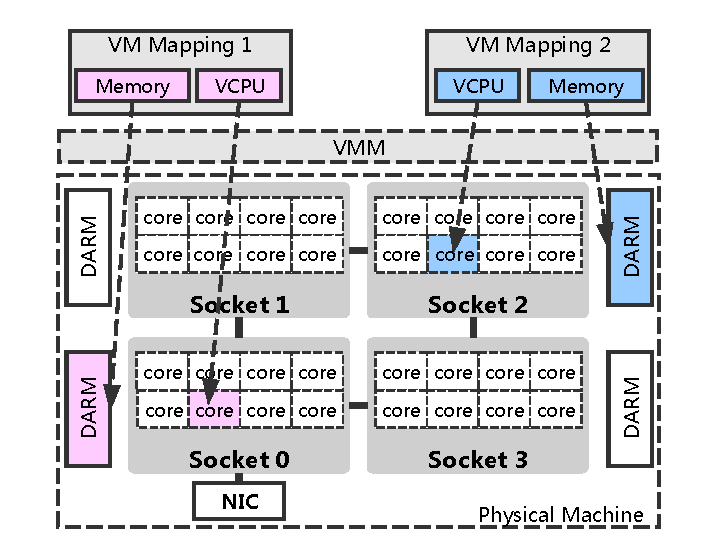
\includegraphics[width=3.5in]{VMmapping1.pdf}
\vspace{-2.0em}
\caption{Different VM mapping strategies based on the asymmetric I/O Access architecture.}
\vspace{-1.0em}
\label{fig_sim}
\end{figure}

Figure 3 gives the performance difference of these two kinds mapping strategies with Intel 10 Gigabit Ethernet adapter and Mellanox 40 Gigabit Ethernet adapter. As for the Intel 10 Gigabit Ethernet adapter, we observe a little bit of throughtput improvement (average 3\%) because the speed of this network adapter can be fully taken advantage of. But for 40 Gigabit network adapter I/O throughtput of first kind of mapping (VM mapping 1)is average 35.1\% (max up to 68.1\%)higher than the I/O throughtput of second kind of mapping (VM mapping 2). The main reason of this huge performance difference is that when transfer data with 40 Gigabit network adapter, the speed of the network adapter is higher than QPI bandwidth. The second kind of mapping need to use two hops interconnection between sockets, this increase the QPI bandwidth consumption and memory access latency, finally, throughput will be decreased.

\begin{figure}[tb]
\centering
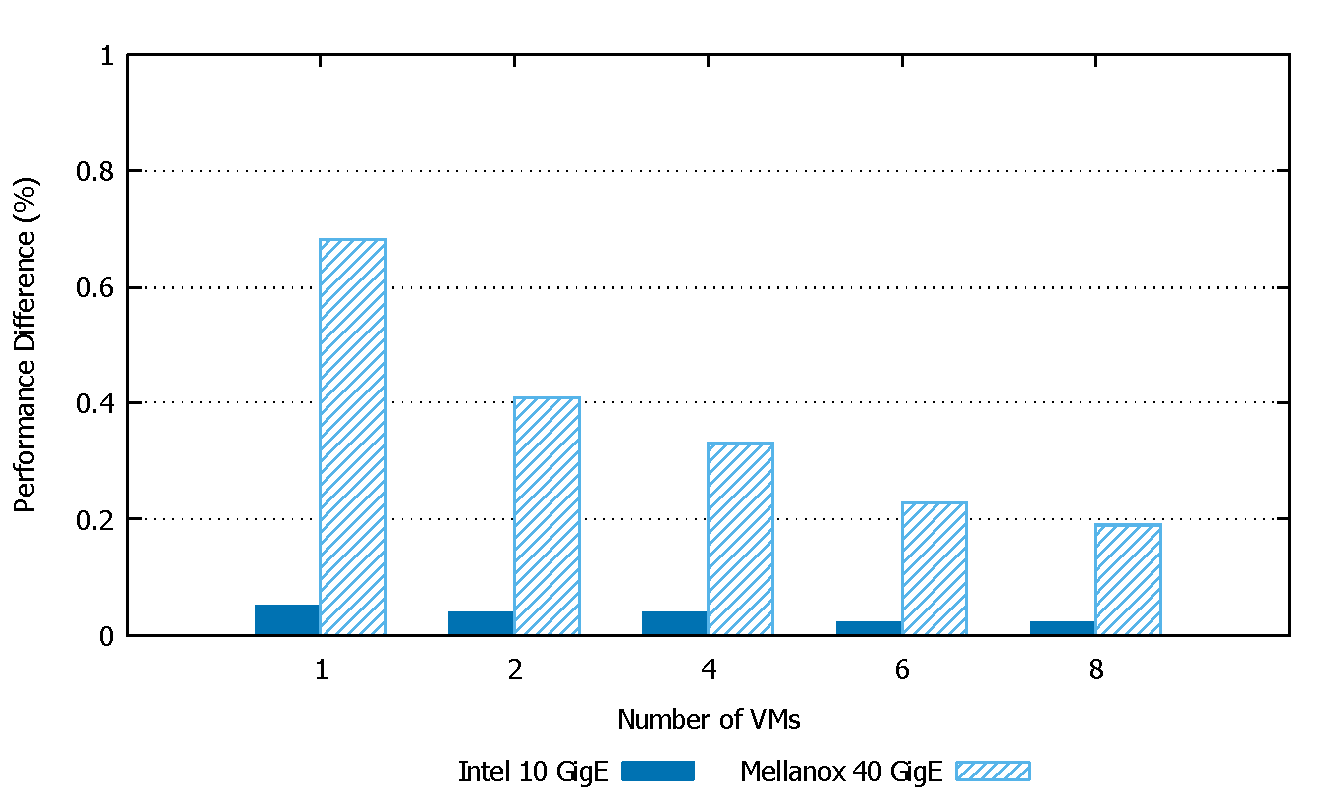
\includegraphics[width=3.2in]{10-40.pdf}
\vspace{-1.0em}
\caption{Performance degradation of different VM mapping strategies (VM mapping 2 relative to VM mapping 1) by using Intel 10 Gigabit Ethernet adapter and Mellanox 40 Gigabit Ethernet adapter.}
\vspace{-1.0em}
\label{fig_sim}
\end{figure}

\subsubsection{Evaluation of Asymmetric I/O Access and Memory Access}
To study the factors of performance degradation in more complex scenarios, we consider the asymmetric I/O access and remote memory access simultaneously. Figure 4 shows three testing scenarios to characterize these two factors. In the Figure 4(A), we bind all the VM vCPUs to the cores on socket 0 and mapping the memory respectively to socket 1, 2 and 3. This scenario ensure all the VM vCPUs in the I/O device attached socket and its memory are remote access. Similar in the Figure 4(B), we consolidate all the VM vCPUs on the socket 1 and mapping the memory respectively to socket 0,2 and 3. This scenario is testing the performance of vCPU binding to the 1-hop distance socket and memory are remote access. Figure 4(C) show the VMs vCPU pining to 2-hops distance socket and memory mapping to socket 0,1 and 3. Not that we do not consider the VM vCPU and memory mapping to socket 3 because of that in our test bed socket 1 and socket 3 are symmetrical.
\begin{figure*}[!t]
\centering
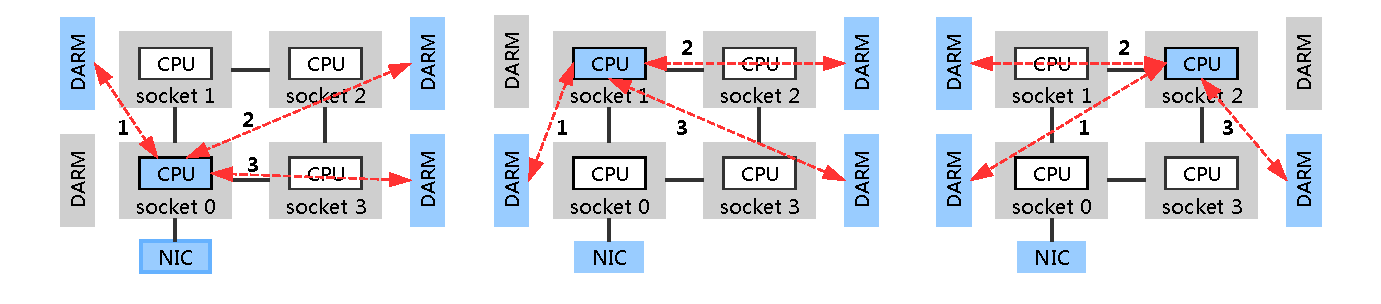
\includegraphics[width=7.0in]{scenario3.pdf}
\vspace{-1em}
\caption{Three scenarios that we use to evaluate performance degradation of the asymmetric I/O access and remote memory access.}
\vspace{-1em}
\label{fig_sim}
\end{figure*}

Figure 5 gives the evaluation results of these three scenarios.


%Papers must be submitted in printable PDF format and should contain a maximum of 11 pages of single-spaced, two-column text, not including references. You may include any number of pages for references, but see below for more instructions.
\subsection{Complexity in Virtualized Systems}
Virtualization poses additional abstraction of the underlying topology and the mapping of VM vCPU and memory in the virtaulized environment is more complexity. This complexity speedup the performance degradation  seriously. Current VMMs tries hard to keep VM memory and vCPU as local as possible (like Xen and VMware ESXi), but mapping between virtual and machine resources must consider all kinds of factors as much as possible and different factors may disturb the distribution of VM vCPUs and memory. According to the white paper of VMware [], the main reason of chaotic mapping in the virtualized system can be listed as follows:
\begin{enumerate}
\item The heterogeneity of the virtual machine will impact the mapping strategies. Different kinds of application running on the VM changes the resources requirement. For example, memory intensive applications running in the virtual machine will result in the VM need lager size of memory, and these large amount of VM memory may distribute across multiple nodes.
\item The load balancing mechanism cause the VM memory and vCPU threads migration. Guest OS shutdown and reboot both trigger load balancing in the host OS, the prior mapping relationship will be changed. This will affect the affinity between vCPU, memory and network adapter. Finally, the system performance degrades.
\end{enumerate}

The asymmetric I/O assess degrade the I/O performance significantly in today's high speed network environment. Virtualization also poses a great challenge for optimizing the affinity among the vCPU, memory and network adapter. These motivate our work and in the next section,we further explore performance degradation in details by a set of experiments.
%Applications running in the virtual machine know little about the physical architecture, resulting in the optimization difficult of virtual machine performance. We should design a efficient virtual machine to physical machine message passing mechanisms.

%\subsection{Challenges in Optimal Performance Modeling}
%Most of current performance models and resource scheduling algorithms focus on the NUMA architecture, but with the emerging of network applications which need huge amounts of I/O operations,these models are no longer suitable. However, to modeling NUIOA architecture in virtualized environment and achieving Optimal Performance is more complicated due to the following challenges:
%
%\textbf{Virtualization poses additional abstraction of the underlying topology:} Applications running in the virtual machine know little about the physical architecture, resulting in the optimization difficult of virtual machine performance. We should design a efficient virtual machine to physical machine message passing mechanisms.
%
%\textbf{Efficient run-time performance monitor for platform independent environment:} The system first must to online monitor the hot page in the virtual machines, I/O request times and system load in the physical machine. These hardware informations are important to our next phase decision, so it must be done efficient and continuously.
%
%\textbf{Frequent migrate thread and memory may incur high overhead:} Because of each VMs vCPU is regarded as a thread in the system, when we migrate the VMs vCPU to other sockets to get optimal performance, the memory of the thread also should be migrated. what's the most important is that migrate such a large amounts of memory can incur high overhead. Thus, we must design efficient and a low overhead thread and memory migrating mechanism and this is challenging because of: 1.migrate a VMs memory always with guest virtual address (GPA) to the host physical address (HPA) translation. 2.we should take system load and threads affinity both into considertion to decide when and how to migrate memory.

%\begin{itemize}
%
%\item If you are using \LaTeX~\cite{lamport94}to typeset your paper, then we strongly recommend that you use the template provided. \textbf{Please set your document to Times font \\ (\texttt{\textbackslash usepackage\{mathptmx\}}) and do not play with interline spacing}.
%
%\item If you are using a different software package to typeset your paper, then please adhere to the guidelines mentioned in the table below. \textbf{You must use 10pt Times font or larger}.
%
%\end{itemize}

%\begin{table}[h]
%\caption{Formatting guidelines.}
%
%\begin{tabular}{ll}
%\hline
%Field &
%Value \\
%\hline
%Page limit &
%11 pages w/o refs. \\
%Paper size &
%US Letter 8.5x11in \\
%Top margin &
%1in \\
%Bottom margin &
%1in \\
%Left margin &
%0.75in \\
%Right margin &
%0.75in \\
%Body &
%2-col., single-spaced \\
%Separation between columns &
%0.25in \\
%Body font &
%10pt Times \\
%Abstract font &
%10pt Times \\
%Section heading font &
%12pt, bold \\
%Subsection heading font &
%10pt, bold \\
%Caption font &
%9pt (minimum), bold \\
%References &
%8pt, no page limit \\
%\hline
%\end{tabular}
%
%\end{table}

%Please ensure that you include page numbers with your submission. This makes it easier for the reviewers to refer to different parts of your paper when they provide comments. Please ensure that your submission has a banner at the top of the title page which contains the submission number and a notice of confidentiality.

\section{Analysis of Optimal Affinity Modeling}
In this section, we begin with the necessity and benefits of modeling the affinity in asymmetric access architecture. We then introduce a set of metrics that can be used to model the affinity in the asymmetric access architecture.
%we conduct a series experiments to study that: 1.virtualization how to affect the performance in current high speed network environment. 2.how the asymmetric I/O access affect the affinity among the VM vCPU, memory and network adapter.
\subsection{Necessity of optimal Affinity Modeling}
\textbf{\emph{Poor Affinity Affect Performance}}: As we experimented and analyzed in the section 2, asymmetric access architecture can not guarantee local access, frequently remote access will cause the performance degradation in high performance networking environment. Nontransparent management in the virtualized system disturb the distribution of all kinds of resources. All these factors finally result in poor affinity among the VM vCPU, memory and network adapter, consequently, the inaccurate affinity model affects the networking performance, poor network performance result in the inefficient of data center servers. Therefore, optimal affinity model in the asymmetric access architecture is necessary.

\textbf{\emph{Inaccurate of Previous Affinity Model}}: Historically, on the one hand, the previous affinity model in the asymmetric architecture mainly focus on optimizing the asymmetric memory access. Undoubtedly, these affinity models are no longer suitable for our asymmetric I/O access affinity modeling. On the other hand, previous affinity models are empirical [], they just characterize the penalty of asymmetric access by using the hop distances. Hop distances are typically recorded as a table in the BIOS Advanced Configuration and Power Interface (ACPI) to measure the distance between NUMA nodes. However, the hop distances lack details in some cases and are insufficient for affinity modeling in asymmetric access architecture.

\subsection{Affinity Classes and Metrics}
We now discuss different affinity classes in the asymmetric access architecture. To accurately determine the affinity among vCPU, memory and network adapter, we adopt more detailed metrics to describe the access behavior in the virtualized systems.

\subsubsection{VCPU to Memory Affinity}
VCPU to memory affinity refers to the traditional NUMA affinity between VM vCPU and its memory. Based on the previous work [], we standing in the point of view of the vCPU and expect the memory access locally as much as possible. The potential for NUMA affinity of vCPU is proportional to the amount of memory access to each NUMA node. That is, if a vCPU access most to the memory of a NUMA node, it has high affinity with this node. The NUMA affinity for vCPU can be calculated with equation 1, where $A_m$ is the affinity between vCPU and each NUMA node n, $NC_k$ is a vector containing the accumulated number of memory access from vCPU k to each node, and N is the number of nodes.
\begin{equation}
A_m=max(NC_k)/(\sum_{i=1}^N NC_k^i)
\end{equation}

This affinity is minimal when the number of memory access from vCPU to each node is equal, in this case, the affinity equal to 1/N. The affinity achieve maximum when all the memory access to one NUMA node, in this caes, NUMA affinity is 1.

\subsubsection{VCPU to NIC Affinity}
The vCPU to NIC affinity is defined as the physical access latency between NIC and the node which vCPU running on. Obviously, the node near to the NIC has best vCPU to NIC affinity. For latency sensitive virtual machines, it is better to binding all their vCPUs to the node near to the network adapter so as to achieve optimal performance. We calculate this affinity with the equation 2, where \emph{delay[N]} is a vector which records the access latency from each node to the NIC, N is the number of NUMA nodes.
\begin{equation}
A_n=max(T_0)/(\sum_{i=1}^N T^m_i)
\end{equation}


\subsubsection{NIC to Memory Affinity}
The NIC to memory affinity is the affinity between NIC ring buffer and VM memory buffer. When a NIC receives incoming packets, it copies the data packets into the buffers using DMA. Obviously, if the DMA buffer is allocated in the memory attached to the node which near to NIC, the access latency of NIC to memory is lowest. Otherwise, NIC access to memory buffer of the remote node by using the QPI link, in this caes, the QPI bandwidth consume quickly. We define the affinity between NIC buffer and memory by using the equation 3, where D is the VM memory distribution table ,$D^m_0$ is memory of virtual machine m distribute on node 0 (which is near to the NIC), and $\sum_{i=1}^N D^m$ is the total number of VM memory.
\begin{equation}
A_b=max(D^m_0)/(\sum_{i=1}^N D^m_i)
\end{equation}

This affinity achieve best when we allocate the VM memory on the node near to the NIC as much as possible.

\subsection{Optimal Affinity Model Function}
After calculate these three classes of affinity metric, we now discuss the optimal affinity model. In consideration of complexity in the virtualized environment, we first simply defined our optimal affinity model function as follows:
\begin{equation}
max\ f(A_m, A_n, A_b)
\end{equation}

As for I/O intensive virtual machines, data interacting with the host machine is frequently. When the NIC receives a large amount of packets, interrupts raising from the NIC also handled by the vCPU of the VM, packets were copied to the memory buffers by using DMA. In this case, the asymmetric I/O accesses are main factors which influencing the performance, our model function focus on optimizing the affinity $A_n$ and $A_b$. As for CPU intensive virtual machine, the vCPU threads frequently access memory to read and write data. In this case, the main factor resulting in the performance degradation is asymmetric memory access, our model function should focus on optimizing the affinity $A_m$.
%\subsection{Experimental Environment}
%different access to directly attached devices affect the performance of the workload in virtualized environment, especially with the different I/O access patten.
%All experiments are conducted in a 4-sockets machine with Mellanox ConnectX-3 40 GigE adapter placed on the PCIe Gen3 x16 slots which directly connect to the socket 0. Each socket contains a Intel Xeon E5 4610 v2(Ivy Bridge architecture) processor and 32GB DDR3 memory bank. Each processor with 8 cores running at 2.3GHz and max turbo frequency can up to 2.7GHz. Each core has 32KB L1 data cache and 32KB L1 instruction cache, 256KB L2 cache and 16MB last level cache (LLC). Each socket equipped with 2 ways QPI with the communication speed 7.2GT/s. In our experiments, we enable the Intel Hyper-threading [](16 logical cores per socket). Therefor, we have total 64 cores and 128GB memory. we also configure the storage with 300G disk, the experiment configuration details are listed in the table 1.
%
%\begin{table}[h]
%\caption{Configuration details of our test server.}
%
%\begin{tabular}{ll}
%\hline
%Item &
%Configuration \\
%\hline
%CPU &
%\tabincell{l}{Intel Xeon E5-4610 v2\\2.3GHz (8 cores)} \\
%\hline
%Memory  &
%128G RAM DDR3 \\
%\hline
%Network Adapter &
%\tabincell{l}{Mellanox ConnectX-3 Dual-Port\\40 Gigabit Ethernet adapter}\\
%\hline
%Hypervisor &
%KVM 2.0.0\\
%\hline
%\end{tabular}
%
%\end{table}

%We use the KVM 2.0.0 as virtual machine monitor with the Intel VT-d and VT-x technology enable. Each VM run the Ubuntu 14.04LTS system and configured with one vCPUs and 1GB memory. In order to achieve high performance I/O virtualization, we enable SR-IOV technology and assigned a virtual function to each VM. We select a set of I/O and memory performance testing benchmarks,listed as table 2. The Netperf [] benchmark provides network bandwidth testing between two host on a network. Memcached [] is an in-memory key-value store for small chunks of arbitrary data to improve the performance of cloud applications.
%\begin{table}[h]
%\caption{Configuration details of our test server.}
%
%\begin{tabular}{ll}
%\hline
%Benchmark &
%Description \\
%\hline
%Netperf &
%\tabincell{l}{Benchmarking the network throughtput \\and delay}\\
%\hline
%YCSB  &
%\tabincell{l}{Benchmarking data read/write/update \\using MySQL database via YCSB interface}\\
%\hline
%\end{tabular}
%
%\end{table}
%Reviewing will be double-blind; therefore, please do not include any author names on any submitted documents except in the space provided on the submission form. You must also ensure that the metadata included in the PDF does not give away the authors. If you are improving upon your prior work, refer to your prior work in the third person and include a full citation for the work in the bibliography. For example, if you are building on your own prior work in the papers~\cite{nicepaper1,nicepaper2,nicepaper3}, you would say something like: ``While prior work did X, Y, and Z~\cite{nicepaper1,nicepaper2,nicepaper3}, this paper additionally does W, and is therefore much better.'' Do not omit or anonymize references for blind review. There is one exception to this for your own prior work that appeared in IEEE CAL, workshops without archived proceedings, etc., as discussed later in this document.

%Recall that, per IEEE authorship guidelines, it is not acceptable to award honorary authorship or gift authorship. Please keep these guidelines in mind while determining the author list of your paper. Also please note that addition/removal of authors once the paper is accepted will have to be approved by the Program Chair.

%\subsection{Evaluation of Degradation}
%To identify and estimate NUIOA system overheads in the virtualized environment, we first run numbers of virtual machines in host machine with the KVM hypervisor, then we design four groups different scenarios by varying memory and vCPUs mappings among these sockets.
%%Ensure that the figures and tables are legible. Please also ensure that you refer to your figures in the main text. Many reviewers print the papers in gray-scale. Therefore, if you use colors for your figures, ensure that the different colors are highly distinguishable in gray-scale.
%\subsubsection{Degradation due to Virtualization}
%As described in the section 2.3, virtualization abstract the underlying hardware resources and present it to the virtual machines. Because of this high level abstraction, the guest OS known inaccurate about the host physical architecture. The VMM must efficiently and accurately translate informations between virtual machines and physical machine. For examples, the virtual CPU(s) need to be mapped into the socket cores and guest OS physical addresses need to translated to machine addresses. But the virtualized resources are not limited to CPU and memory, high speed I/O devices are also generally virtualized. If VMMs don not carefully take underlying topology into consideration, the performance could not be optimizing and system overheads increasing.
%
%Current VMMs like Xen, VMware ESXi and KVM, to keep local access by allocating all the memory of a VM to one NUMA node and migrate the vCPU threads to this node. This method is inefficient in today's high performance virtualized system due to following two reasons:
%\begin{itemize}
%  \item Some memory intensive applications running in the VM need large size of memory, when the VMs memory larger than the total socket memory bank, it have to be assign memory to other sockets. Similarly, while computing intensive applications need multiple VM vCPUs, also causing cross sockets mapping.
%  \item The system load balancing mechanism will cause the memory and vCPU migration. Guest OS shutdown and reboot both trigger load balancing in the host OS, the prior mapping relationship will be changed. This will affect the system performance.
%\end{itemize}
%
%In order to show the original I/O performance in the current virtualized environment,we simply run numbers of virtual machines without any memory and vCPU binding. Figure 4 show that
%
%\subsubsection{Degradation due to NUIOA}
%I/O devices as a very important resource in the computer system. Each VM has its own virtualized I/O devices and mapping to the physical machine. Previous works mainly focus on I/O virtualization to improving virtualized I/O devices performance. Currently, because of the speed of I/O devices become higher and higher, non-uniform I/O access bring new overheads. We evaluate these overheads by following for groups experiments.
%
%In the Figure 3(A), we binding VMs vCPU and memory together to the same socket to ensure memory is local access and testing the different socket I/O performance. For example, we deploy all VMs on the socket 0 by pining these VMs vCPU to the cores in the socket 0 and mapping VMs memory to the memory banks directly attached to the socket 0 (marked in red). Similarly, we test the performance of socket 1 (marked in yellow),socket 2 (marked in blue) and socket 3 (marked in green). In the Figure 3(B), we bind all the VMs vCPU to the socket 0 and mapping the memory respectively to socket 1 and socket 2. This scenario ensure all the VMs vCPU in the I/O device attached socket and its memory are remote access. Similar in the Figure (C), we consolidate all the VMs vCPU on the socket 1 and mapping the memory respectively to socket 0,2 and 3. This scenario is testing the performance of vCPU binding to the 1-hop distance socket and memory are remote access. Figure 3(D) show the VMs vCPU pining to 2-hops distance socket and memory mapping to socket 0 and 1. Not that in the Figure 3(B) and 3(D) we do not consider the socket 3 because of that in these two scenarios socket 1 and socket 3 are symmetrical. These four scenarios can testing all combination cases among the vCPU, memory and I/O devices.
%
%Figure 4 shows the normalized performance of our test results. Figure 4(A) shows that
%\begin{figure*}[!t]
%\centering
%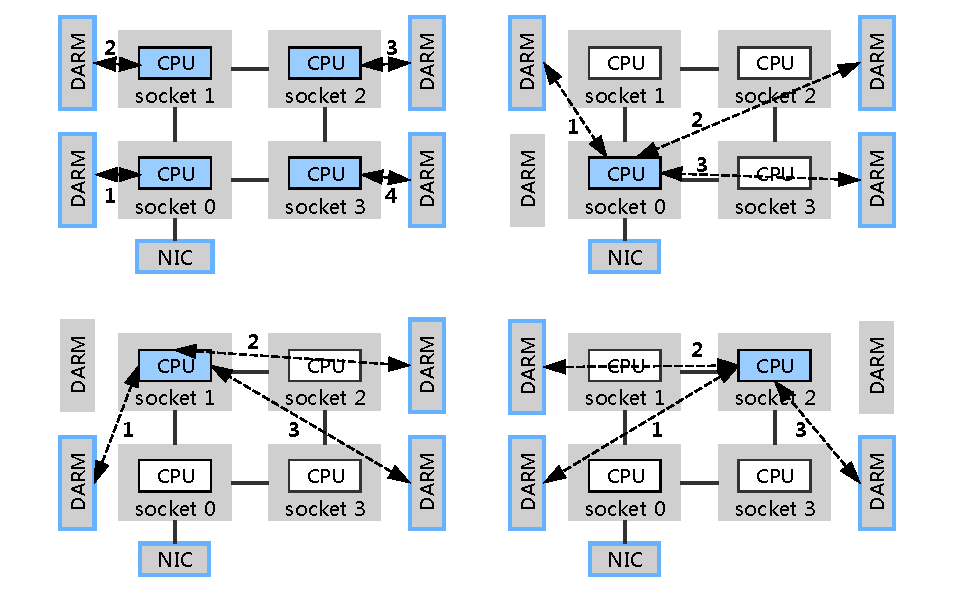
\includegraphics[width=7.0in]{Test-scen.pdf}
%\vspace{-1em}
%\caption{Four scenarios that we use to characterize NUIOA architecture overheads.}
%\vspace{-1em}
%\label{fig_sim}
%\end{figure*}
%
%\begin{figure*}[!t]
%\centering
%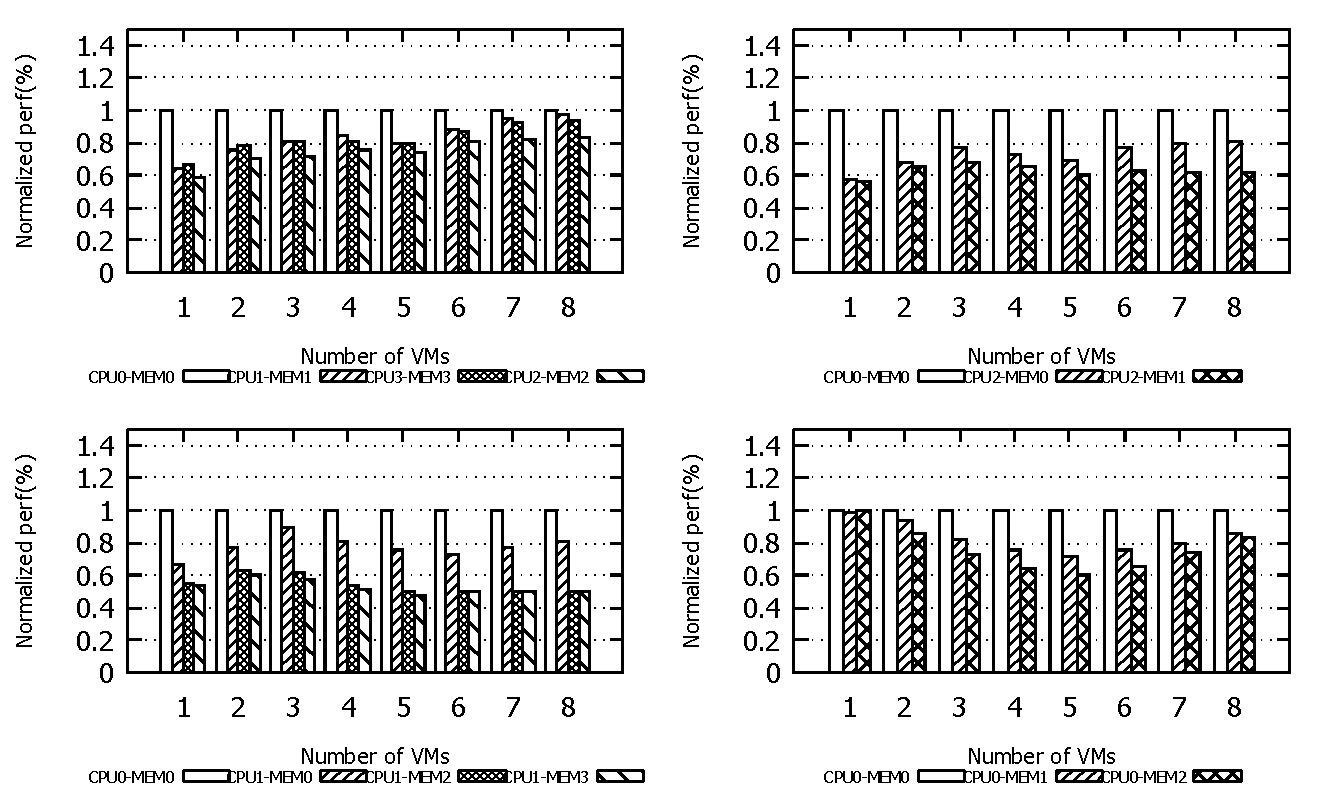
\includegraphics[width=7.0in]{Test2.pdf}
%\vspace{-1em}
%\caption{Testing results.}
%\vspace{-1em}
%\label{fig_sim}
%\end{figure*}

\section{Design}
In this section, we describe the detail design of our vNUIOA, a platform independent runtime system that optimizing the overheads of asymmetric access architecture. We enabling three parts for incorporating NUMA and NUIOA overheads awareness with hypervisor: namely, Runtime information collector, Affinity aware algorithm and Dynamic load balance scheduler.

\subsection{Overview}
An overview of vNUIOA is shown in Figure 5. It consists of the following three parts: the \textbf{\emph{Runtime Access Analyzer}} modules collects guest os and host server information since the system booting, then the module classify and store these information of each VM. After these information is collected, we design the asymmetric access overheads awareness algorithm based on the optimal affinity model which describe in the section 3.

%If the system load is not balanced and a certain node's load is very high, we should going to the \textbf{\emph{ threads affinity manager}} module and using I/O intensive aware migration strategy to migrate the VM vCPU threads to the appropriate NUMA node. Otherwise, the system load is balanced, we will going to the \textbf{\emph{memory affinity manager}} module to optimizing the memory affinity and achieving high performance.

\begin{figure*}[!t]
\centering
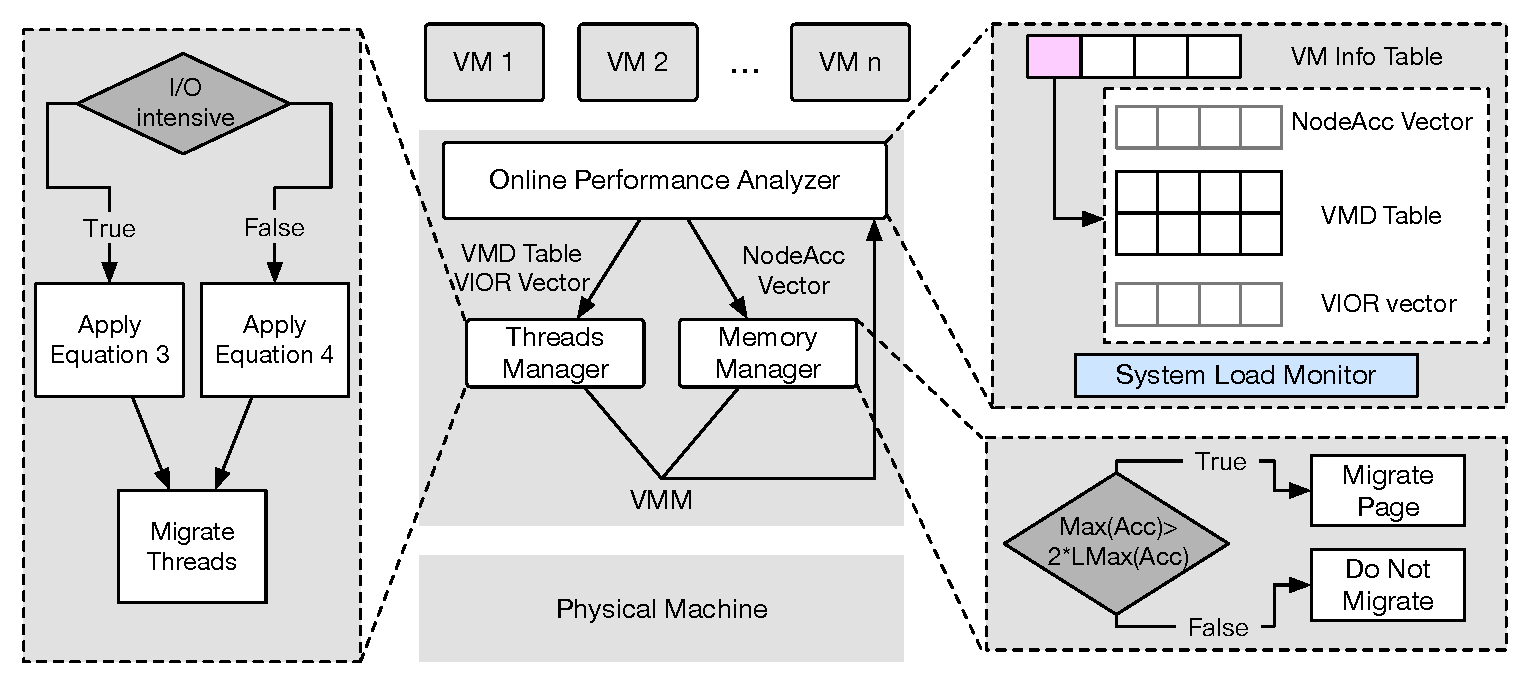
\includegraphics[width=7.0in]{VNUIOA-Arch.pdf}
\vspace{-1em}
\caption{Architecture of vNUIOA .}
\vspace{-1em}
\label{fig_sim}
\end{figure*}

\subsection{Runtime information collector}
Runtime information collector mainly collects the information we used in the optimal affinity modeling. To periodically collect the performance information of virtual machines and host server, it is imperative to analyze memory and I/O access activities in the virtualized system. To end this, we use the Linux performance monitoring tool perfmon [] to detect each virtual machine's memory and I/O access activities,then we store these information in the VMinfo table. Each table entry contains information about each NUMA node access to VM pages vector(NodeAcc Vector), VM memory distribution table (VMD table) and VM I/O request times vector (VIOR Vector). The detail of these three information listed as follows:
\begin{table}[h]
\caption{Definitions of collected information.}

\begin{tabular}{|l|l|}
\hline
\multicolumn{2}{|c|}{Per VM statistics}\\
\hline
NC vector &
\tabincell{l}{NC[n] records the accumulated \\ number of memory access from VM \\vCPU to each NUMA node.} \\
\hline
VMD table &
\tabincell{l}{VMD[m][n] table describe the VM m\\ memory distribute to each node n}\\
\hline
VIOR vector  &
\tabincell{l}{VIOR[m] vector records the number of \\I/O requests per second for VM m.}\\
\hline
\hline
\multicolumn{2}{|c|}{Physical machine statistics}\\
\hline

\end{tabular}
\end{table}



%\begin{itemize}
%  \item \textbf{NodeAcc vector}: The \emph{NodeAcc[n][p]} records the number of memory access from node n to each page p of the VM. The OS has a methods to measure if the pages has been accessed by the page fault, While the page is not set as present in the page table, the OS is noticed about the faulting virtual address, as well as the thread ID that caused the fault. By tracking page faults, it possible to detect which vCPU threads are accessing the memory page. We apply this memory access vector to vCPU thread to memory affinity modeling.
%  \item \textbf{VMD table}: The VM memory distribution table, denoted as \emph{VMD$\left[m\right]\left[n\right]$}, collects the number of VM m memory references to NUMA node n. We analysis the VM guest physical address (GPA) and translate it to host physical address (HPA). Based on the HPA, we can obtain the distribution of virtual machine memory to the physical server nodes. The VMD table provide data distribution information for our NIC to vCPU thread affinity modeling.
%  \item \textbf{VIOR vector}:The virtual machine I/O request times vector records the I/O request times per second. This information used to identify whether the virtual machine is I/O intensive. If the I/O operations of a virtual machine are too frequent, we should take a special consideration of these kinds of virtual machine in the NIC to vCPU thread affinity modeling.
%\end{itemize}

System load balance is also important for performance of physical server. As shown in the section 3.2.1, physical machine system load imbalance will cause a huge performance degradation. So in our design, we must take the system load into consideration. In this paper, we mainly consider two kinds of system load of each NUMA node,the per-node CPU load \emph{NCL$_n$} and the per-node memory load \emph{NML$_n$}. These two kinds of load can be calculate as follows:
\begin{equation}
L_n=NCL_n+NML_n
\end{equation}
we test that when the system load per node exceed the $80\%$ of the max load, the system performance begin to goes down. Based on this experimental value, if the system load per node up to $80\%$, the load of the node is high.

Because of the hop-distance result in the previous NUMA affinity modeling inaccurate, in this work, we use a more accurate system information for NUIOA affinity modeling. We measure the average access latency between NIC and every NUMA node ,then we record it in a ACL vector (\emph{ACL[n]}). Based on the ACL vector, the data transfer latency between NIC and nodes can be accurate measured and we this information in the following affinity modeling.
\subsection{Affinity aware algorithm}
\textbf{Step 1}: we first identify which type a virtual machine belong to, because for different type VM, we adopt different optimal function to manage affinity. We classify the VMs into I/O intensive and I/O non intensive by looking the VIOR vector(see the Table 2), the I/O request threshold is to be determined experimentally. We found that the number of I/O request for VM with running CPU intensive task is less than 100 per second and for I/O intensive task the number is more than 1000 per second, so we choose a threshold value of 500 times per second in consideration of practical application attributes.

\textbf{Step 2}:calculating the optimal affinity for each VM. For different type of virtual machine, we assign different weight to the three affinity $A_m, A_n, A_b$, in this way, we can figure out optimal affinity function. I/O intensive VMs always have frequent I/O operation, so the affinity $A_n, A_b$ are more important in the optimal function, and as a result, the weight of the $A_n, A_b$ is dominant. CPU intensive VMs always read and write data with memory, in this case, the proportion of affinity $A_m$ is higher in the optimal function and we should assign a proper weight.

\textbf{Step 3}: According to the calculating results in the step 2, we make the decision of memory migration and vCPU remapping. we only migrate memory when maximum number of remote node memory access is double than the number of local memory access (\emph{max(NC)>2*NC[0])}, because frequent memory migration also bring high overheads. We test several value and found that when select 2 times than the number of local access, we can achieve max benefits. The vCPU remapping also negotiate with the load balance mechanism in the system, the load of cpu core i can be calculated by $L_i=\frac{CPUtime_i}{Elapsedtime_i}$. If the average CPU load per node is higher than 80\%, we should not map any vCPU to this node and select node with low load and calculate optimal once more.

%(\emph{$\sum_{i=1}^M L_i / M > 80\% $})





\subsection{NUIOA Affinity Modeling}
We now discuss the affinity modeling of NUIOA architecture. NUIOA affinity measure the Based on the evaluation of performance degradation in the section 3, we divide the entire affinity modeling into two parts: the NIC to VCPU Threads Affinity Modeling and the VCPU Threads to Memory Affinity Modeling.

\subsubsection{NIC to vCPU Thread Affinity Modeling}
The NIC to vCPU thread affinity model mainly measure the affinity between NIC and vCPU thread running in each NUMA node. After the VM system boots up, we first To optimize the mapping of vCPU threads to the processing cores on the NUMA node, VM vCPU affinity manager periodically receive the VIOR vector and VMD table from the performance analyzer. We also periodically update these information per second to reduce the influence of old values.

The I/O intensive virtual machine always have frequent I/O operation and the asymmetric I/O access hurt the system performance significant,so we must give priority to calculating the I/O intensive vCPU threads mapping. We first identify whether the virtual machine is I/O intensive by looking the value in the VIOR vector. Previous research [] has shown that the I/O request of CPU intensive is less than 100 times per second and I/O intensive is more than 1000 time per second, so we choose a threshold value of 500 times per second in consideration of practical application
attributes. Once the number of I/O request exceeds the threshold, the VM is regarded as I/O intensive. After classify these VM threads by using the threshold, we first migrate I/O intensive VM vCPU threads to the node near to high performance network adapter according to the equation 2.

\begin{equation}
Aff_{THR}[n]=\frac{VMD[m][n]}{\sum_{i=1}^n VMD[m][i]}ACL[n]
\end{equation}

Where the $Aff_{THR}[n]$ is the VM affinity vector of the NIC to each NUMA node. \emph{VMD[m][n]} is the number of VM m memory distribute in node n and \emph{$\sum_{i=1}^n VMD[m][i]$ }is total number of VM m memory. \emph{ACL[n]} is the access latency from the NIC to node n. We can regard this affinity as the distance of NIC to the node and it is more accurate than the hop-distance.

If this mapping result in the load imbalance, then we should calculate remapping strategy of the VM vCPU threads to other nodes by using the NIC to vCPU thread affinity model:

\begin{equation}
remapping=\begin{cases}
true& \text{$if Aff_{THR}[k] >Aff_{THR}[p]$}\\
false& \text{otherwise}
\end{cases}
\end{equation}

This equation implies that remapping the VM m vCPU thread from the original node to node k instead of the node p is beneficial only if the affinity to node k is better than affinity to node p.

\subsubsection{VCPU Thread to Memory Affinity Modeling}
VCPU thread to memory affinity modeling is deigned to model the affinity between vCPU thread and VM memory. We first identify which page of a VM are frequently accessed by calculating the access number of every memory page. After obtain the NodeAcc table from the performance analzyer, we calculate the $Aff_{MEM}$ vector for each VM by following equation:
\begin{equation}
Aff_{MEM}[n]=\sum_{p=1}^m NodeAcc[n][p]
\end{equation}
We use the total number of memory access from vCPU thread to NUMA node measure the vCPU thread to memory affinity. $Aff_{MEM}[n]$ is the VM total access number to each other node n which VM original running on. For example, NodeAcc[0] is the total local access number and NodeAcc[1] is the total number of memory access to node 1). If the number of remote access to a node is double than the number of local access, the page in the remote node will be migrate to the local node. Equation 4 formalizes this behavior, where  max($Aff_{MEM}[n]$) is the highest number of remote access and the NodeAcc[0] is number of local memory access.

\begin{equation}
Migrate=\begin{cases}
true& \text{if max($Aff_{MEM}[n]$)>2*$Aff_{MEM}[0]$}\\
false& \text{otherwise}
\end{cases}
\end{equation}

The reason why we select double than the number of local access is that frequent memory migration also bring high overheads. We test several value and found that when select 2 times than the number of local access, we can achieve max benefits.
%There is no length limit for references. Each reference must explicitly list all authors of the paper. Papers not meeting this requirement will be rejected.

\section{Implementation}
We implemented the vNUIOA prototype in the KVM virtualized platform. The online performance analzyer, the threads migration manager and the memory migration manager are implemented as individual daemous in the KVM system. We describes the implementation details of these three modules.

We use the KVM 2.0.0 as virtual machine monitor with the Intel VT-d and VT-x technology enable. Each VM run the Ubuntu 14.04LTS system and configured with one vCPUs and 1GB memory. In order to achieve high performance I/O virtualization, we enable SR-IOV technology and assigned a virtual function to each VM. We select a set of I/O and memory performance testing benchmarks,listed as table 2. The Netperf [] benchmark provides network bandwidth testing between two host on a network. Memcached [] is an in-memory key-value store for small chunks of arbitrary data to improve the performance of cloud applications.

\subsection{Techniques for Information Collection}
\textbf{\emph{Using page faults measure memory accesses}}: The OS has a methods to measure if the pages has been accessed by the page fault, While the page is not set as present in the page table, the OS is noticed about the faulting virtual address, as well as the thread ID that caused the fault. By tracking page faults, it possible to detect which vCPU threads are accessing the memory page. The performance analyzer accesses the hardware performance counters via Linux performance monitor tool \emph{perfmon}. We using

\textbf{\emph{Counting I/O requests per second}}: As for the number of I/O request per second, we count the execution number of $ixgbevf\_clean\_tx\_irq$ or $ixgbevf\_clean\_rx\_irq$ function for every second. Because every time a VM handles a packet, the SR-IOV vf driver invokes these two functions.

\textbf{\emph{Migrating pages via system call}}: After determine memory migration, we use the \emph{numa\_migrate\_pages()} system call to migrate all pages of the specified process from one node to another node. This system call supported by \textbf{libnuma} in the \textbf{numactl} package.


\subsection{Threads Migration Manager}

\subsection{Memory Migration Manager}

\section{Evaluation}
In this section we present experimental evaluation of the proposed vNUIOA system, we compare the performance of vNUIOA with KVM's default scheduler and a hand-optimized binding strategy. Then we study the stability of our vNUIOA system. Finally, we characterize vNUIOA runtime overhead.

\subsection{Experimental Environment}
%different access to directly attached devices affect the performance of the workload in virtualized environment, especially with the different I/O access patten.
All experiments are conducted in a 4-sockets machine with Mellanox ConnectX-3 40 GigE adapter placed on the PCIe Gen3 x16 slots which directly connect to the socket 0. Each socket contains a Intel Xeon E5 4610 v2(Ivy Bridge architecture) processor and 32GB DDR3 memory bank. Each processor with 8 cores running at 2.3GHz and max turbo frequency can up to 2.7GHz. Each core has 32KB L1 data cache and 32KB L1 instruction cache, 256KB L2 cache and 16MB last level cache (LLC). Each socket equipped with 2 ways QPI with the communication speed 7.2GT/s. In our experiments, we enable the Intel Hyper-threading [](16 logical cores per socket). Therefor, we have total 64 cores and 128GB memory. we also configure the storage with 300G disk, the experiment configuration details are listed in the table 1.


\subsection{Improvement of Performance}
\subsection{}
\section{Related work}

\section{Conclusion}
%Authors must register all their conflicts on the paper submission site. Conflicts are needed to ensure appropriate assignment of reviewers. If a paper is found to have an undeclared conflict that causes a problem OR if a paper is found to declare false conflicts in order to abuse or ?game? the review system, the paper may be rejected.

%Please declare a conflict of interest with the following people for any author of your paper:

%\begin{enumerate}
%\item Your Ph.D. advisor(s), post-doctoral advisor(s), Ph.D. students, and post-doctoral advisees, \textbf{forever}.
%\item People (including students) who shared your primary institution(s) \textbf{in the last five years}.
%\item People with whom you have collaborated \textbf{in the last five years}, including:
%\begin{itemize}
%\item Co-authors of papers whether accepted, rejected, pending, or in preparation.
%\item Co-PIs on funding proposals whether accepted, rejected, pending, or in preparation.
%\end{itemize}
%\item Decision-makers of your research funding whether current, pending, or in preparation, and researchers whom you fund.
%\item Other relationships, such as family relations by blood or marriage or their equivalent (if they might be potential reviewers), close personal friendships, etc., that may be reasonably perceived as influencing judgment by a person aware of the relationship.
%\end{enumerate}

%``Service'' collaborations, such as co-authoring a report for a professional organization, serving on a program committee, or co-presenting tutorials, do not themselves create a conflict of interest. Co-authoring a paper that is a compendium of various projects with no true collaboration among the projects does not constitute a conflict among the authors of the different projects.
%
%We hope to draw most reviewers from the PC and the ERC, but others from the community may also write reviews. Please declare all your conflicts (not just restricted to the PC and ERC). When in doubt, contact the Program Chair.

\section{Prior/Concurrent Submissions}

%By submitting a manuscript, the authors guarantee that the manuscript has not been previously published or accepted for publication in a substantially similar form in any conference, journal, or the archived proceedings of a workshop (e.g., in the ACM digital library); but see exceptions below. The authors also guarantee that no paper that contains significant overlap with the contributions of the submitted paper will be under review for any other conference or journal or an archived proceedings of a workshop during the review period. Violation of any of these conditions will lead to rejection.
%
%The only exceptions to the above rules are for the authors? own papers in (1) workshops without archived proceedings such as in the ACM digital library (or where the authors chose not to have their paper appear in the archived proceedings), or (2) venues such as IEEE CAL where there is an explicit policy that such publication does not preclude longer conference submissions. In all such cases, the submitted manuscript may ignore the above work to preserve author anonymity. This information must, however, be provided on the submission form, as the Program Chair will make this information available to reviewers if it becomes necessary to ensure a fair review. As always, if you are in doubt, it is best to contact the Program Chair.
%
%Finally, we also note that the ACM Plagiarism Policy covers a range of ethical issues concerning the misrepresentation of other works or one's own work; please consult it carefully.

%%%%%%% -- PAPER CONTENT ENDS -- %%%%%%%%

%%%%%%%%% -- BIB STYLE AND FILE -- %%%%%%%%
\bibliographystyle{ieeetr}
\bibliography{ref}
%%%%%%%%%%%%%%%%%%%%%%%%%%%%%%%%%%%%

\end{document}
